%----------------------------------------------------------------------------------------
%	PACKAGES AND OTHER DOCUMENT CONFIGURATIONS
%----------------------------------------------------------------------------------------

\documentclass[11pt]{article}
\usepackage{hyperref}
\usepackage{listings}
\usepackage{caption}
\usepackage{subcaption}

\input{structure.tex} % Include the file specifying the document structure and custom commands

%----------------------------------------------------------------------------------------
%	ASSIGNMENT INFORMATION
%----------------------------------------------------------------------------------------

% Required
\newcommand{\assignmentQuestionName}{} % The word to be used as a prefix to question numbers; example alternatives: Problem, Exercise
\newcommand{\assignmentClass}{Zero to ASIC} % Course/class
\newcommand{\assignmentTitle}{Analogue Design} % Assignment title or name
\newcommand{\assignmentAuthorName}{Thomas Parry} % Student name





% Optional (comment lines to remove)
%\newcommand{\assignmentClassInstructor}{Jones 10:30am} % Intructor name/time/description
%\newcommand{\assignmentDueDate}{Monday,\ January\ 24,\ 2019} % Due date

%----------------------------------------------------------------------------------------

\begin{document}

%----------------------------------------------------------------------------------------
%	TITLE PAGE
%----------------------------------------------------------------------------------------

\maketitle % Print the title page

\thispagestyle{empty} % Suppress headers and footers on the title page

\newpage


\section{Fundamentals of the MOSFET}

The MOSFET (Metal-Oxide Semiconductor Field Effect Transistor) is the fundamental building block of modern IC design.

\begin{figure}[h]
\centering{
\includegraphics[scale=1.00]{diagrams/nmos.pdf}
}
\end{figure}

The MOSFET is a \textit{transconductance} device which translates a voltage between it's gate and source terminals to a current between the drain and source - assuming the device is biased correctly.

\subsection{The Saturation Region}

Most devices in a circuit will be operating in saturation where the following description of the current is given for a square-law device:

\begin{equation}
I_D = \frac{1}{2} \mu_n C_{ox} \frac{W}{L} {\left( V_{GS} - V_{TH} \right)}^2
\end{equation}

This can be simplified to:

\begin{equation}
I_D = K_n \frac{W}{L} {V_{OD}}^2
\end{equation}

\begin{equation}
given \; that: \;\;\; V_{DS} > V_{OD}
\end{equation}

The condition is very important, if you want your FET to work as expected you must ensure you have sufficient $V_{DS}$ headroom.  The value $V_{OD}$ is also more commonly called $V_{D_{SAT}}$ and is defined as the minimum drain voltage required to keep the device in saturation. Note that in sub-micron processes (like Skywater 130 nm) the statement that $V_{D_{SAT}} = V_{OD}$ is not fully accurate due to second order effects from device scaling.


\subsection{The Triode Region}

When there is insufficient drain-source voltage (by design or error) the device will work in the triode region where it approximates a voltage controlled resistor:

\begin{equation}
I_D = \mu_n C_{ox} \frac{W}{L} \left( (V_{GS} - V_{TH}) V_{DS} - \frac{V_{DS}^2}{2} \right)
\end{equation}

\subsection{The Cutoff Region}

When there is insufficient voltage across the gate-source terminals the device is 'off':

\begin{equation}
I_D = 0 \;\;\;\; given \; that: \;\; V_{GS} << V_{TH}
\end{equation}


\answer{Always know the region you expect your FET to operate and check that you have it correctly biased or all other assumptions are broken.}

\section{Basics of Transconductance Efficiency}

The transconductance is the amount of current in the drain per gate-source voltage.

\begin{equation}
i_d = g_m \cdot v_{gs}
\end{equation}

This simple diagram shows the most important concept of the FET: a voltage at the input is converted to an output current. This output current will later be converted by an impedance to another voltage.

\begin{figure}[h]
\centering{
\includegraphics[scale=1.00]{diagrams/nmos_smallsignal.pdf}
}
\end{figure}


The transconductance can be expressed as a function of the bias current, giving the $g_m / I_d $ value. This value is related to how inverted the channel of the FET is - a measure of how 'turned on' the FET is. The measure of channel inversion is how many minority charge carriers have been attracted to the conductive channel between the source and drain.

\subsection{Transconductance Efficiency and Overdrive Voltage}

There is a relation to the overdrive voltage mentioned above, $V_{OD}$. The higher the $V_{OD}$, the more the FET is 'turned on', and therefore the more the FET channel is inverted, which leads to a \textit{lower} $g_m / I_d$. Conversely, a lower $V_{OD}$ turns on the FET less, and therefore the FET channel is less inverted, which leads to a \textit{higher} $g_m / I_d$.

\subsection{Realistic Values of Transconductance Efficiency}

There is a range of transconductance efficiencies that can be obtained in standard CMOS processes. It is reasonable to assume a maximum transconductance efficiency of 20 in design equations, although in some specific cases values of 25 can be reached. Typically a device will not be used below a transconductance efficiency of 4.

\subsection{Why Use Transconductance Efficiency?}

While transconductance efficiency, $g_m/I_d$, feels very abstract at first, its use lies in two factors.

\begin{enumerate}
  \item It gives a strong indication of the channel inversion.
  \item It allows quick calculation of circuit currents and other conditions.
\end{enumerate}

For example, if I have determined I will use a FET in weak inversion and I need $1 \; mS$ of transconductance, then I very simply know the required current of $50 \; \mu A$.

\answer{But how do we know what transconductance we should use for a given FET? We'll discuss this in the next section where I will talk about the relation of matching and noise to transconductance.}

\textbf{Further Reading (clickable)}

\hspace{1cm} \href{http://web02.gonzaga.edu/faculty/talarico/EE406/documents/gmid.pdf}{gm/ID - Based Design}

\hspace{1cm} \href{http://web.eecs.utk.edu/~bblalock/ece532/ece532_pres_ekv_bsim.pdf}{An Introduction to the EKV Model and a comparison of EKV to BSIM}

\newpage
\section{Noise, Offset and Transconducance}

\subsection{Noise}

Considering only thermal noise the drain noise in a MOSFET is given by:

\begin{equation}
\frac{i^2_{n,d}}{\Delta f} = 4 K T \gamma g_{do}
\end{equation}

Where the $ K $ is the Boltzmann's constant and $T$ is absolute temperature. We will set the device specific parameter $\gamma=1$ for simplicity. The zero bias drain conductance, $g_{do}$, can be approximated to $ g_m $.

\begin{equation}
\frac{i^2_{n,d}}{\Delta f} \approx 4 K T g_{m}
\end{equation}

So now we can see that the current noise in the drain of a MOSFET \textbf{increases} with increasing transconductance. However, to complete the story we can also refer the noise to the gate. To do this we divide the noise power above by the power transfer function of the MOSFET, $g^2_{m}$, to give:

\begin{equation}
\frac{v^2_{n,d}}{\Delta f} \approx \frac{4 K T}{ g_{m} }
\end{equation}

Now we see that expressed as a input referred noise source the noise \textbf{decreases} with increasing $g_{m}$. This is because the increasing gain of the MOSFET overpowers the increasing noise in the channel. The result also complies with the intuition formed by Friis' equation.


\subsection{Offset}

All MOSFETs are fabricated with random variations which exhibit as mismatch offset between ideally identical devices. The largest contributor to offset is due to the gate-source threshold voltage offset. Pelgrom proposed the following model for offset which is widely adopted:

\begin{equation}
\sigma_{\Delta V_{TH}} = \frac{A_{VTH}}{\sqrt{WL}}
\end{equation}

This states that the standard deviation of the mismatch between two devices is a process specific value divided by the square root of the area of the device (assuming both devices are identical). The SKY130 process does not have a published figure for $A_{VTH}$ but using $10 \ mV \mu m$ is reasonable.

Consider the small signal description of the FETs transfer:

\begin{equation}
i = g_m \cdot v_{GS}
\end{equation}

Where we then add an offset:

\begin{equation}
i = g_m \cdot ( v_{GS} + \Delta V_{TH} )
\end{equation}

We can see that the offset voltage is transferred to the current as a function of $g_m$. So for small drain current offset we need a low $g_m$.

Considering a voltage amplilfier, the original threshold offset cannot be improved but any offset further down the system can be modelled as input referred but divided by $g_m$. Therefore, we want a high $g_m$, this tracks with Friis' equation.


\newpage
\section{The Current Mirror}

The most important circuit in analogue design is the current mirror. This circuit is used as the building block for a huge amount of applications.

\begin{figure}[h]
\centering{
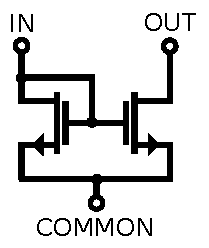
\includegraphics[scale=1.00]{diagrams/current_mirror.pdf}
}
\end{figure}

\subsection{Circuit Operation}

The input current is fed into a diode-connected FET. This diode-connected FET generates a voltage on it's gate which is approximately equal to:

\begin{equation}
V_{GS} = \sqrt{I_{IN} \frac{1}{K_n} \frac{L}{W}} + V_{TH}
\end{equation}

This voltage is then applied to the gate of the second FET. Assuming the sizes are the same, the output current will then match the input current. If the sizes are different then the output current is scaled by:

\begin{equation}
I_{OUT} = {\left(\frac{W}{L}\right)}_{OUT} \cdot {\left(\frac{L}{W}\right)}_{IN}
\end{equation}

To have good matching performance usually $L_{IN} = L_{OUT}$ and $\frac{W_{OUT}}{W_{IN}} $ is a rational number so that unit FETs can be used.

\subsection{Selecting Sizes}

How do we select the value of $\frac{W}{L}$? As we discussed previously the output is a current so to get the best performance for thermal noise and offset we need to use a low $g_m$. This means we need a low transconductance efficiency where the channel is heavily inverted and the overdrive voltage is high.

To achieve this, generally we want a low value of $\frac{W}{L}$. Although the absolute value depends on the device used, PMOS devices have a lower charge mobility than NMOS so will require a higher $\frac{W}{L}$ ratio. Aim for a $g_m/I_d$ of 5-7 or a $V_{DS,sat}$ of 300 - 350 mV.

\newpage
\section{The Differential Pair}

The differential pair is shown below. It is most commonly seen at the input of op-amp circuits but is also seen in many other places.

\begin{figure}[h]
\centering{
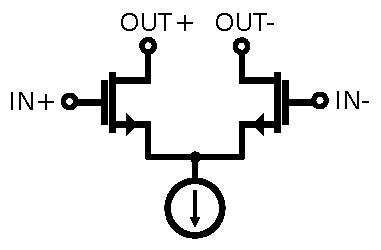
\includegraphics[scale=1.00]{diagrams/differential_pair.pdf}
}
\end{figure}


\subsection{Circuit Operation}

The differential pair compares two voltages and splits the bias current depending on the difference between the input voltages. 

If the two input voltages are equal then $V_{GS}$ is equal for both devices and both devices get half of the bias voltage. If $V_{IN+}$ is higher than $V_{IN-}$ then more current flows into $V_{OUT+}$ and less into $V_{OUT-}$, but the sum still remains the same bias current.

\subsection{Selecting Sizes}

As already discussed in the section on noise and offset the differential pair devices should operate with a high $g_m$ and therefore a high transconductance efficiency. Therefore the ratio of $\frac{W}{L}$ should be high. Aim for a $g_m/I_d$ of 20-25 or a $V_{DS,sat}$ of 10 - 50 mV.

\newpage
\section{Useful Circuits}

\subsection{Transmission Gate}

A building block switch made of one or more FETs. The control signals are digital and the terminals $A$ and $B$ are analogue.

\begin{figure}[h]
\centering{
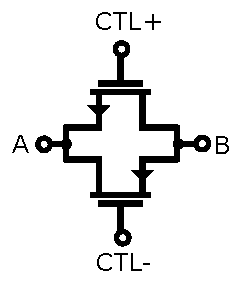
\includegraphics[scale=1.00]{diagrams/transmission_gate.pdf}
}
\end{figure}

Important factors:

\begin{itemize}
  \item On resistance of switch
  \item Charge injection
\end{itemize}


\subsection{5T Op-Amp}

A simple two stage op-amp circuit with differential inputs and current output. Stability can be improved with a Miller capacitor across the output stage.

\begin{figure}[h]
\centering{
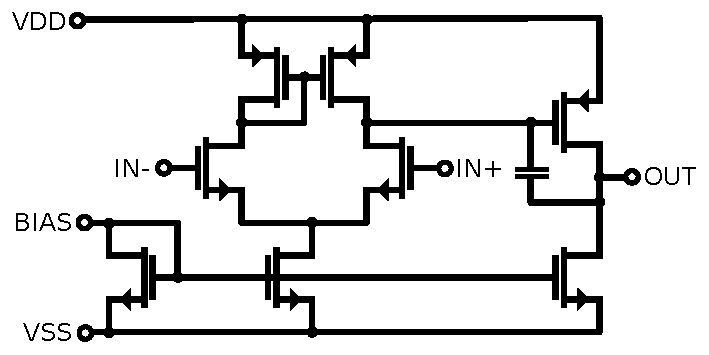
\includegraphics[scale=1.00]{diagrams/opamp_5t.pdf}
}
\end{figure}

Important factors:

\begin{itemize}
  \item Input/Output Voltage Ranges
  \item Gain
  \item Bandwidth
  \item Stability
  \item Noise
  \item Slew Rate
\end{itemize}



\newpage
\section{Opamp Verification}

There are a number of standard verification measurement points for an op-amp circuit. Some of the later half may be skipped if they are not particularly important in the circuits application. The first half must be performed to have reasonable confidence in the operation of the circuit.

\begin{table}[h]
\resizebox{\textwidth}{!}{%
\centering
\begin{tabular}{llll}
\textbf{Name}      & \textbf{Conditions}           & \textbf{Sim} & \textbf{Description} \\ \hline
Operating Point    & min/max($V_{IN}$/$V_{OUT}$)   & .op          & Ensure all devices are operating in correct region (usually saturation) \\
AC Gain            & min/max($V_{IN}$/$V_{OUT}$)   & .ac          & Simulate AC gain of opamp \\
AC Stability       & min/max($V_{IN}$/$V_{OUT}$)   & .ac          & Simulate phase/loop gain \\
Tranient Stability & small $V_{IN}$ step           & .tran        & Observe transient stability in response to a step function \\
Offset             & min/max($V_{IN}$)             & .dc          & In unity gain what is the input referred offset \\
Slew Rate          & large $V_{IN}$ step           & .tran        & Put opamp into large signal slew and ensure it meets requirements \\
Noise              & min/max($V_{IN}$/$V_{OUT}$)   & .noise       & Simulate input referred noise performance \\
PSRR               & min/max($V_{IN}$/$V_{OUT}$)   & .ac          & Simulate Power Supply Rejection Ratio \\
CMRR               & min/max($V_{IN}$/$V_{OUT}$)   & .ac          & Simulate Common Mode Rejection Ratio \\
\end{tabular}}
\end{table}

These would be repeated in a number of conditions progressively as the design matures:

\begin{itemize}
  \item Typical corner
  \item Across all corners
  \item Monte-Carlo random sampling
\end{itemize}

The typical corner is where the main design phase occurs, ensuring the main functional performance is as expected. Once the circuit works well in a typical conditions, the full range of environmental and manufacturing conditions need to be explored. This is normally achieved by simulating over PVT (Process, Voltage and Temperature). Usually there are five MOS corners (tt, ff, fs, sf, ss) plus passive corners, the voltage range is commonly the nominal supply +/-10\% and temperature depends on application - for commercial $0 - 85^\circ C$ is acceptable.

Once these verification points have been covered and documented the circuit is ready to move to layout.

\newpage
\section{Layout}

Once the schematic has been fully investigated the layout phase can begin to describe the physical implementation on silicon.

\subsection{Wells}

In a bulk CMOS process (like SKY130) everything is built into a common substrate with differently doped regions. Typically the substrate is P- doped before the device fabrication begins.

An NMOS consists of a channel which is P- doped and N+ doped drain/source. As the electrostatic potential of the gate inverts the region below the gate with negative charge carriers (electrons) a conductive channel is formed.

\begin{figure}[h]
\centering{
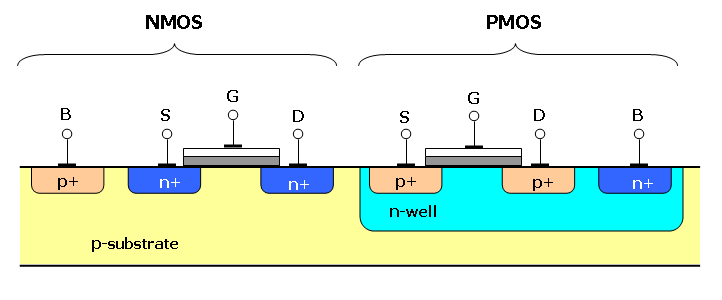
\includegraphics[scale=0.50]{diagrams/cmos_well.png}
}
\end{figure}


To create PMOS devices a N- bulk is required. To achieve this a well is created in the substrate where PMOS devices can be created. An NWELL is defined and many PMOSs can be manufactured within it. It is very important to note that the NWELL is a PN junction with the substrate which forms a diode. If the NWELL is biased at a lower potential than the substrate a current will begin to flow.

\subsubsection{Latchup}

Once the PMOS devices have been created a structure exists which can be very destructive. The drain/source of the PMOS is P, the bulk N, the P substrate and the N drain/source of the NMOSs. This structure can form a parasitic thyristor structure with positive feedback which once triggered allows very high currents to flow causing damage to the device.


\begin{figure}[h]
\centering
\begin{subfigure}{0.6\textwidth}
  \centering
  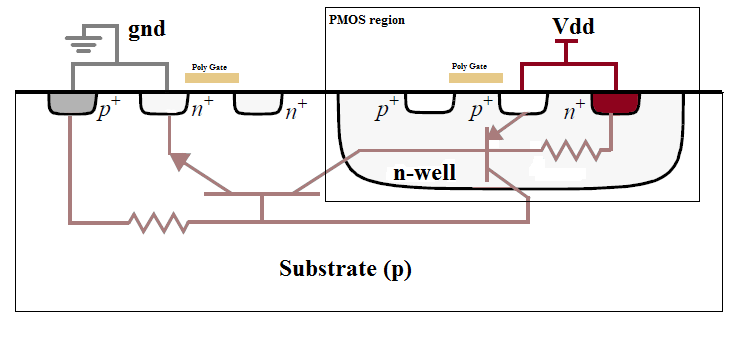
\includegraphics[width=1.0\linewidth]{diagrams/latchup_layout.png}
  \caption{layout}
\end{subfigure}%
\begin{subfigure}{0.4\textwidth}
  \centering
  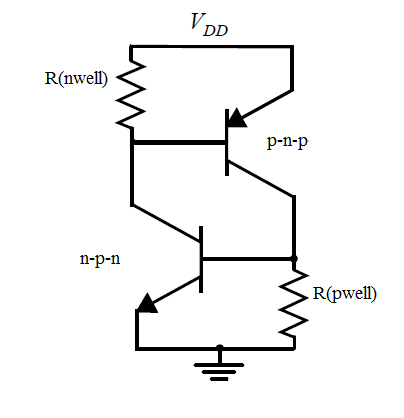
\includegraphics[width=0.6\linewidth]{diagrams/latchup_circuit.png}
  \caption{circuit}
\end{subfigure}
\end{figure}

The likelihood of latchup occurs primarly as a function of voltages applied between PN junctions, the parasitic bulk resistors and bipolar gains. To prevent latchup these causes should be dealt with in that order.

The easiest way to prevent latchup is ensure that the PN junctions never get biased. This is achieved by ensuring the bulk is always at a lower potentional than any sources (for NMOS). The second step is to reduce parasitic resistors which bias the thyristor. This is achieved by reducing the distance between sources and bulk connections.

\subsubsection{Triple Well}

The NMOS devices can be fabricated directly into the bulk substrate but they all share a common bulk which must be connected to the lowest potentional, usually ground. This can be an issue for two main reasons. If the circuit requires the bulk of NMOSs to be connected to their source - commonly to prevent body effect in differential pairs - this is not possible with substrate based NMOSs. Secondly all the NMOS devices share a common connection, there is a bulk resistance between all NMOSs in the IC. This is very bad for interference between circuits, for example switching digital and sensitive analogue receivers. To alleviate these problems some processes provide a triple-well process. Here a deep NWELL is created in the P substrate, then another PWELL is created inside the DNWELL. NMOS devices can then be created in the new PWELL which is isolated from the P substrate.

\begin{figure}[h]
\centering{
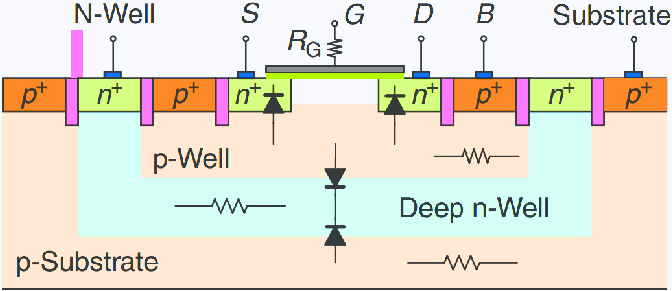
\includegraphics[scale=1.00]{diagrams/triple_well.png}
}
\end{figure}

Now another level of PN junctions have been created which need to be carefully biased to ensure that currents don't flow which can cause latchup. A representation of the distrubted diodes in a triple-well NMOS is shown below.


\begin{figure}[h]
\centering{
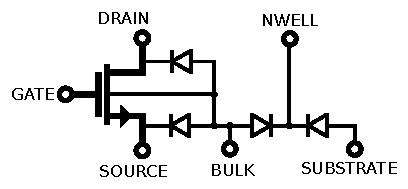
\includegraphics[scale=1.00]{diagrams/nmos_triplewell.pdf}
}
\end{figure}



\subsubsection{Contact Rings}

One of the most effective layout techniques to ensure high performance is the use of contact rings into the substrate and wells. The rings ensure that a strong connection to the bulk potentional is created. It also helps reduce interference coupling between different sections of the IC by creating lower impedance sinks or minority charge collectors depending on the relative doping of the rings.

It is good practise to place a continous contact ring around all wells, collections of devices and the overall block in the substrate.

\begin{figure}[h]
\centering{
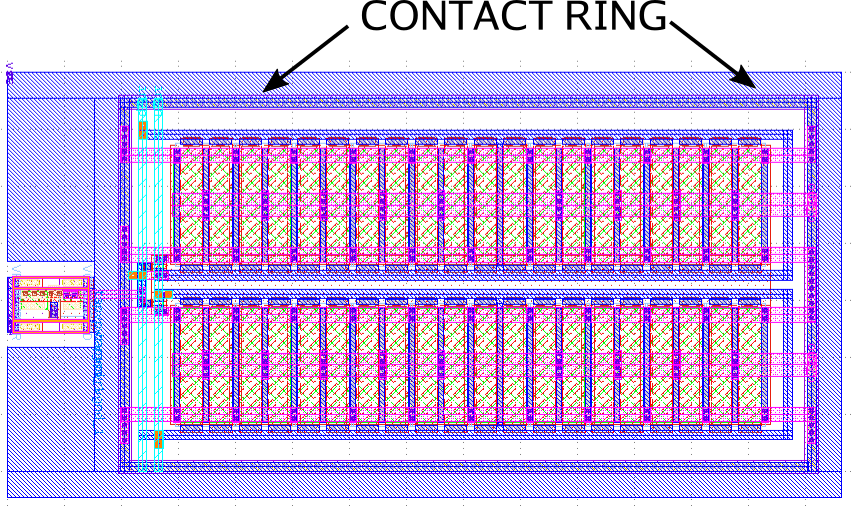
\includegraphics[scale=0.5]{diagrams/contact_rings.png}
}
\end{figure}


\subsubsection{Practical Notes On Wells}

The layout and structure of the wells is the bedrock that the circuit is created in. Ensure you have a plan for the wells arrangement before you begin. The spacing of wells can also have a large impact on the layout size and arrangement. This is especially true for triple wells which require a large spacing to avoid punchthrough under higher voltages.






\newpage
\section{NGSpice Notes}

\subsection{Saving Operating Parameters}

To save the operating parameters in NGSpice outputs the following syntax needs to be used:

\begin{lstlisting}
    .save all @M.x1.XMcas_p.msky130_fd_pr__pfet_01v8[vdsat]
\end{lstlisting}

The addition of all is to prevent NGSpice \textit{only} saving operating parameter and none of the voltages. Note that the string starts with an M for MOSFET then the dot delimited path to the transistor model. The exact transistor model needs to be used. Finally the operating parameter can be specified in square brackets. This is reqiured for every device and paramter you want to investigate.

Some common parameters:

\begin{lstlisting}
    gm vdsat vds id
\end{lstlisting}


\end{document}
